%% Important points

%% \begin{enumerate}
%% \item Pointer safety and Pool Containment
%%   \begin{enumerate}
%%   \item No null pointer dereference (Rust)
%%   \item No inter-pool pointers \nameref{inv:no-interpool-ptrs}
%%   \item No NV-to-V pointers \nameref{inv:no-v-pointers}
%%   \end{enumerate}
%% \item Transactions
%%   \begin{enumerate}
%%   \item Atomicity \nameref{inv:tx-atomic}
%%   \item Consistency \nameref{inv:inevitable-logging}
%%   \item Isolation (Rust)
%%   \item Durability ***
%%   \item all of the above for volatile data too.
%%     \begin{enumerate}
%%     \item Atomicity \nameref{inv:tx-no-volatile-mutability}
%%     \item Consistency \nameref{inv:inevitable-logging}
%%     \item Isolation (Rust)
%%     \end{enumerate}
%%   \end{enumerate}
%% \item Memory safety
%%   \begin{enumerate}
%%   \item No memory leaks. \nameref{inv:no-orphans}
%%   \item No multiple frees. \nameref{inv:correct-gc}
%%   \end{enumerate}
%% \item Concurrency
%%   \begin{enumerate}
%%   \item No data races. (Rust)
%%   \item No unsynchronized access. (Rust)
%%   \end{enumerate}
%% \end{enumerate}

%auto-ignore
\lstMakeShortInline^

\section{\This}
\label{sec:overview}

\This{} is a Rust library (or ``crate'') that uses static and dynamic checking to avoid common PM programming errors.
Aside from providing these strong safety guarantees, \this{} 
is similar to other PM programming libraries like
PMDK~\cite{pmdk}, NV Heaps~\cite{nvheaps}, and Mnemosyne~\cite{mnemosyne}.
\This{} provides four abstractions -- typed persistent memory pools,
transactions, persistent smart pointers, and atomic memory allocation -- that
address the challenges and common bugs described in \refsec{sec:prog}.

\This{} strives to provide strong safety guarantees for persistent memory programming.
It achieves the following design goals:


%% \begin{itemize}

%%   \myitem{Transactions and Atomic Memory Management} All modification to
%%   persistent data (including memory allocation) occur within transactions.
%%   \This{} enforces this constraint statically making a pool's journal object
%%   available inside transactions and no where else.

%%   \ignore{\This{} enforces this constraint by requiring all mutating,
%%     allocating, and deallocating operations to take a journal object (of type
%%     \csym{Journal<P>}) as a parameter.  Journal objects are only available
%%     inside transactions and cannot escape.}

%%   \myitem{Leak-Free Memory Allocation} To prevent persistent memory leaks,
%%   \this{} statically ensures that, by the end of the enclosing transaction, any
%%   allocated memory has either been reclaimed or been made reachable from the
%%   root of the memory pool.

%%   \myitem{Logging errors} Journal objects record mutating operations made during a
%%   transaction, so they can roll back in case of a system failure or
%%   transactions abort.  Since all mutating operations require a journal object,
%%   it is not possible to accidently omit an update from the journal.

%%   \myitem{Inter-pool pointers} Since the type of each persistent pointer and
%%   object includes a pool type, \this{} can prevent inter-pool pointers by
%%   disallowing assignments between different pool types.
  
%% \end{itemize}


%% \begin{enumerate}
%% \item Pointer safety and Pool Containment
%%   \begin{enumerate}
%%   \item No null pointer dereference (Rust)
%%   \end{enumerate}
%% \item Transactions
%%   \begin{enumerate}
%%   \item Atomicity \nameref{inv:tx-atomic}
%%   \item Consistency \nameref{inv:inevitable-logging}
%%   \item Isolation (Rust)
%%   \item Durability ***
%%   \item all of the above for volatile data too.
%%     \begin{enumerate}
%%     \item Atomicity \nameref{inv:tx-no-volatile-mutability}
%%     \item Consistency \nameref{inv:inevitable-logging}
%%     \item Isolation (Rust)
%%     \end{enumerate}
%%   \end{enumerate}
%% \item Memory safety
%%   \begin{enumerate}
%%   \item No memory leaks. \nameref{inv:no-orphans}
%%   \item No multiple frees. \nameref{inv:correct-gc}
%%   \end{enumerate}
%% \item Concurrency
%%   \begin{enumerate}
%%   \item No data races. (Rust)
%%   \item No unsynchronized access. (Rust)
%%   \end{enumerate}
%% \end{enumerate}


\begin{goal}[Only-Persistent-Objects]
  Pools only contain data that can be safely persistent.\label{goal:only-persistent-objects}
\end{goal}
\begin{goal}[Ptrs-Are-Safe]
  Pointers within a pool are always valid.  Pointers between pools or from
  persistent memory to volatile memory are not possible.  Pointers from
  volatile memory into a pool are safe.  Closing a pool does not result in
  unsafe pointers.\label{goal:ptrs-are-safe}
\end{goal}
\begin{goal}[Tx-Are-Atomic]
  Transactions are atomic with respect to both persistent and volatile data.
  It is not possible to modify persistent data without logging
  it.\label{goal:atomic-is-atomic}
\end{goal}
\begin{goal}[No-Races]
  There are no data races or unsynchronized access to shared persistent data. \label{goal:no-races}
\end{goal}
\begin{goal}[Tx-Are-Isolated]
  Transactions provide isolation so that updates are not visible until the transaction commits. \label{goal:atomic-is-isolated}
\end{goal}
\begin{goal}[No-Leaks]
  Memory leaks and multiple frees are not possible. \label{goal:no-memory-leaks}
\end{goal}
%\begin{goal}[No-NV-to-V-Ptr]
%  \This{} pools do not contain pointers to volaitle memory.  \label{goal:no-pool-to-dram-ptr}
%\end{goal}
%\begin{goal}[V-to-P-Ptrs-Are-Safe]
%  \This{} pools do not contain pointers to volaitle memory.  \label{goal:no-pool-to-dram-ptr}
%\end{goal}
%\begin{goal}[Inevitable-Logging]
%  Modifying data without logging the change is not possible. \label{goal:inevitable-logging}
%\end{goal}
%\begin{goal}[No-Null-Deference]
%  Null pointer derefence is not possible. \label{goal:no-null-dereference}
%\end{goal}

\This{} achieves these goals through a combination of several core techniques
that are embodied by \this{}'s abstractions.  \This{} borrows and relies
upon existing features of Rust to prevent data races and avoid unsafe pointer
manipulation.  These properties are a foundation that \this{} builds upon.

\this{} breaks a program's execution into transactions and non-transactional
code, and a thread's execution alternates between the two.  Transactions are atomic,
isolated, and can modify persistent state but cannot modify pre-existing
volatile state.  The remaining, non-transactional code
can modify volatile state but cannot modify persistent state.

Critically, \this{} limits the kinds of variables that can cross transaction
boundaries, and this allows for careful reasoning about the invariants that
hold at the boundaries.  For instance, \this{} guarantees that leaks are not
possible by showing that they do not exist at transaction boundaries.

\subsection{Assumptions}

\ignore{The correctness of \this{} builds on many features of Rust and its safety
properties.  In particular we rely directly on Rust to satisfy two of our
design goals: \nameref{goal:no-memory-leaks} and \nameref{goal:no-races}.  The
Rust documentation~\cite{rustbook} details of how Rust provides these
guarantees.}

The correctness of \this{} rests on several assumptions.
We assume that the program does not use \csym{unsafe} constructs, since
unsafe Rust can bypass almost all of the guarantees that Rust makes and relies
upon.  \ignore{\This{} also prohibits spawning threads inside a transaction, for reasons discussed in \refsec{sec:discuss}.}

We also assume that our implementation of the \this{} memory allocator,
logging and recovery code, and reference counting system are correct.  We have
tested them thoroughly and techniques for building correct versions of these
components are well-known~\cite{nvheaps,mnemosyne,atlas,pmdk,oracle-nvm-direct}.

Finally, students of Rust will notice that we do not discuss some common types
(e.g., \csym{Cell} or \csym{Weak}) or their persistent analogs.
\This{}'s treatment of these types is analogous to the types we discuss and \this{}
provides persistent counterparts.  We have omitted the details for brevity.

\subsection{\This{} Pools and Objects}

\This{} provides self-contained pools of persistent memory and constrains the
data types that they can hold.

\boldparagraph{Pools} \This{} pools reside in a
PM-backed file.  The pool contains some metadata, a root pointer, persistent
memory allocation data structures, and a region of persistent memory.

\This{} identifies each memory pool with a \emph{pool type}, and all persistent
types take a pool type as a parameter.  This statically binds each persistent
object to its pool.  Likewise, transactions are bound to a particular pool via
the pool type.  In our discussion, we use \csym{P} as a representative pool
type.

Programs open a pool by calling \csym{P}'s \cfunc{open} function: \csym{P::open<T>(foo)}.  This binds \csym{P} to the pool in file
\csym{foo}.  \This{} ensures that only one open pool is bound to \csym{P} at
any time.  The type parameter, \csym{T}, determines the type of the root
pointer.  \cfunc{P::open<T>} returns an immutable reference to the root pointer.  Pools remain
open until the reference to the root object drops.

Programmers can statically declare multiple pool types using the
\cfunc{Pool!} macro, but the number of pool types available (and,
therefore, the number of simultaneously open pools) is fixed at compile time.

\boldparagraph{Persistent Objects} Objects in a pool must implement the
\csym{PSafe} auto trait.  \This{} declares all primitive arithmetic types to be
\csym{PSafe}, so these types and structs composed of them are \csym{PSafe}.

\csym{PSafe} (like all of \this{}'s auto traits) is declared
\csym{unsafe}, so programmers should not explicitly label types as \csym{PSafe}
or \csym{!PSafe}.

Reference and smart pointer types that point to volatile data (e.g.,
references, mutable reference, \csym{Box}, \csym{Arc}, \csym{Rc}, and
\csym{Mutex}) and types that refer to state external to the program (e.g., file
handles) are \csym{!PSafe}.

\subsection{Transactions: The Basics}

\begin{lstfloat}
  \begin{lstlisting}[escapechar=\@]
#[derive(Root)]
struct Node {
  val: i32,
  next: PRefCell<Option<Pbox<Node,P>@@>,P>
}
fn append(n: &Node, v:i32, j: &Journal<P>) {
  let mut t = n.next.borrow_mut(j);@\label{ln:borrow}@
  match &*t {@\label{ln:match}@
    Some(succ) => append(succ, v, j);
    None => *t = Some(Pbox::new(@\label{ln:new}@
        Node {
          val: v,
          next: PRefCell::new(None, j)
        }, j));
  }
}
fn go(v: i32) {
  let head = P::open::<Node>("list.pool",0);
  P::transaction(|j| {@\label{ln:tx}@
    append(&head, v, j);@\label{ln:call}@
  });@\label{ln:txend}@
}
\end{lstlisting}
\caption{A \this{} implementation of linked list append.  Some error management code has been elided for clarity.}
\label{lst:example}
\end{lstfloat}

% \begin{table*}%[!ht]
%   \center
%   \small
%   \begin{tabular}{p{3.4in}p{3.4in}}
%     \begin{lstlisting}[escapechar=\#,caption=Insert method of a sorted linked-list in Rust]
% struct Node {val:i32, nxt:Rc<RefCell<Option<Node>>>}
% impl Node {
%   fn append(&self, val: i32) {
% #\hllr{\linewidth}#
%     let mut nxt = self.nxt.borrow_mut();
%     if let Some(n) = &*nxt {
%       if n.val > val {
%         *nxt = Some(Node { val,
%           nxt: self.nxt.clone()
%         })
%       } else { n.insert(val); }
%     } else {
%         *nxt = Some(Node { val,
%           nxt: Rc::new(RefCell::new(None))})
%     }
% #\hllr{\linewidth}#
%   }
% }
% fn main() {
% #\hllr{\linewidth}#  let head = #\hlc{77pt}#Default::default();
%   head.insert(10);
% }\end{lstlisting}
%     &
%       \begin{lstlisting}[escapechar=\#,caption=Insert method of a sorted linked-list in \This,label=lst:examples]
% #\hll{\linewidth}# struct Node {val:i32, nxt:#\hlw{12pt}#Prc<#\hlw{32pt}#PRefCell<Option<Node>>>}
% impl Node {
%   fn append(&self, val: i32) {#\label{ln:tx2}#
% #\hll{\linewidth}#    #\hlw{72pt}#transaction(|j| {
% #\hll{\linewidth}#      let mut nxt = self.nxt.borrow_mut(#\hlw{5pt}#j);#\label{ln:borrow}#
%       if let Some(n) = &*nxt {#\label{ln:if}#
%         if n.val > val {#\label{ln:if2}#
%           *nxt = Some(Node { val,
% #\hll{\linewidth}#            nxt: self.nxt.#\hlw{38pt}#pclone(j)
%           })
%         } else { n.insert(val); }
%       } else {
%         *nxt = Some(Node { val,
% #\hll{\linewidth}#          nxt: #\hlw{12pt}#Prc::new(#\hlw{32pt}#PRefCell::new(None,#\hlw{5pt}#j),#\hlw{5pt}#j)})#\label{ln:new}#
%       }
% #\hll{\linewidth}#    #\hlw{47pt}#}).unwrap()#\label{ln:txend2}#
%   }
% }
% fn main() {
% #\hll{\linewidth}#  let head = #\hlw{127pt}#P::open::<Node>("list.pool",0);
%   head.insert(10);
% }\end{lstlisting}
% \end{tabular}
% \vspace*{-\baselineskip}\vspace*{-\baselineskip}
% \end{table*}


All modifications to a \this{} pool occur within a transaction, including
memory allocations and modifications of the root pointer.

Programs create transactions by passing an anonymous function (i.e., a lambda) to \cfunc{P::transaction} (\reflr{ln:tx}{ln:txend} of \reflst{lst:example}).
The lambda takes a single
argument, \csym{j}, which will be reference to a \emph{journal object} that holds information about the current transaction.  Variable
\csym{j} is of type \csym{Journal<P>}, so it is bound to pool \csym{P}.  

The lambda can capture values from the transaction's lexical scope (e.g., \csym{head} in \reflst{lst:example}), allowing
transactions to integrate smoothly into the surrounding code.
\cfunc{P::transaction} returns the return value of the transaction body.

\This{} flattens nested transactions: Modifications to a
pool commit when outermost transaction for that pool commits.  \cutforspace{This rule
holds for nested transactions on different pools, so an inner transaction on
\csym{P} will commit before an enclosing transaction on \csym{Q} finishes.   We discuss
the possibilities for multi-pool transactions in \refsec{sec:discuss}.}

The programmer is responsible for acquiring locks in the correct order to avoid deadlock.

Rust's type system allows \this{} to restrict the inputs and output of the
transaction.  The \csym{TxInSafe} auto trait bounds the types a transaction
can capture.  \This{} marks all volatile mutable references, smart pointers, wrappers,
and interior mutability types as \csym{!TxInSafe}.

This provides our first invariant:

\begin{invar}[TX-No-Volatile-Mutability]
  \label{inv:tx-no-volatile-mut}
  Transactions cannot modify existing volatile state.
\end{invar}

\begin{discuss}
  Since all the types that provide mutable access to volatile data are
  \csym{!TxInSafe}, pre-existing instances of these variables are not available
  inside the transaction.  However, new instances of these variables can be created and
  modified within the transaction.  Preexisting volatile data can be read.
  
\cutforspace{The code below illustrates the restrictions. The transaction can declare
volatile variables on the stack or heap inside the transaction (\reflr{l:createvstart}{l:createvend}),
modify them, and read captured values (\reflr{l:modifyvstart}{l:modifyvend}).
But, it cannot modify captured values (\reflr{l:unsaferef}{l:unsafebox}).  Nor
can it create a mutable reference to a captured value (\refl{l:unsafemake}).

\ignore{\begin{lstlisting}
    let mut a = 42;
    let b = &mut a;
    let mut c = Box::new(42); 
    let r = P::transaction(|j| {
	let mut d = 0;             #\label{l:createvstart}#
	let mut e = Box::new(42);  #\label{l:createvend}#
	d = a;  #\label{l:modifyvstart}#
	*e = a; #\label{l:modifyvend}#
        // #\rerr{}#*b = 0;  #\label{l:unsaferef}#
        // #\rerr{}#*c = 0;  #\label{l:unsafebox}#
        // #\rerr{}#let g = &mut a; #\label{l:unsafemake}#
	// #\rerr{}#return e #\label{l:noreturnbox}#
	return d #\label{l:yesreturnvalue}#
    }).unwrap();
\end{lstlisting}}
}

\cutforspace{The example shows that the transaction can return newly-created volatile data
by value (\refl{l:yesreturnvalue}) but not by reference/pointer (\refl{l:noreturnbox}).}

%% \subsubsection{Durability.} Another aspect of pointer safety is that the objects they refer live longer than the static lifetime of the program, and they should be reachable when the program restarts to avoid memory leaks. Therefore, \this{} prevents moving out a pointer wrapper from the transaction that it is born in, unless there is a link from the root object to it. To implement that, we consider a special auto trait `\csym{TransactionOutSafe}' that is not implemented by the pointer wrappers. Then we bound the output types of the transaction to be marked as \csym{TransactionOutSafe}.

%% \begin{lstlisting}[caption={Persistent pointer lifetime},label={lst:lifetime}]
%% let p1 = P::transaction(|j|{
%%     let p1 = Pbox::new(1, j);
%%     let p2 = Pbox::new(2, j);
%%     root.set(p2);
%%     p1
%%     --^^ the trait bound `Pbox<i32,P>: 
%%     --TransactionOutSafe` is not satisfied
%% }).unwrap();
%% ++^ `p1` is dropped here.
%% ++^ `p2` is alive and durable here because it
%% ++  is reachable from the root object.
%% \end{lstlisting}
%% }

%Since newly-allocated volatile memory cannot escape, it will be reclaimed when
%the transaction ends.  As a result,

\end{discuss}



\csym{TxOutSafe} bounds the values a transaction can return.  All references
and pointers are \csym{!TxOutSafe}, so transactions can return data only by
value.

\This{} also uses the concept of a \emph{stranded type}: If a type is
\csym{!TxOutSafe}, \csym{!Send}, and \csym{!PSafe}, then instances of that type
cannot escape a transaction.  This is because 1) Since a stranded type is
\csym{!TxOutSafe}, the transaction cannot return it, 2) since it is
\csym{!PSafe}, it cannot be stored in a pool for later retrieval, 3) since it is
\csym{!Send}, it cannot be passed to another thread, and 4) it cannot be assigned 
to a volatile variable (\nameref{inv:tx-no-volatile-mut}).

%\This{} uses is this capability to enforce several invariants:

\begin{goaltrue}{goal:only-persistent-objects}
  The declaration of \cfunc{P::open} includes a bound to ensure that the root is
  \csym{PSafe}.  If it contains references or pointers they must be one of
  the persistent reference/pointer types (see below), since volatile pointers
  and references are \csym{!PSafe}.
  
  \csym{PSafe} is a type bound on all of the persistent smart pointer and wrapper
  types, so those types can only point to, refer to, or wrap \csym{PSafe}
  objects.
\end{goaltrue}

\This{} also carefully constrains the availability of journal objects:

\ignore{\begin{invar}[TX-No-PMEM-Return]
  \label{inv:tx-no-pmem-return}
  Transactions cannot return pointers or references to persistent data.
\end{invar}

\begin{discuss}
  \This{} marks all persistent pointer, reference, and wrapper types as \csym{!TxOutSafe}.
\end{discuss}
}

\begin{invar}[TX-Journal-Only]
  \label{inv:tx-journal-only} 
  Journal objects are only available inside transactions.  \cutforspace{For nested
  transactions, only the journal object for the innermost transaction is
  available.}
\end{invar}

\begin{discuss}
  The constructor for the \csym{Journal<P>} is unsafe, so the program cannot
  safely create one.  Therefore, the only journal objects that might be
  available are the ones passed to a transaction as an argument.
  \csym{Journal<P>} is declared to be stranded, so it cannot escape the transaction.
  
  \cutforspace{Finally, a nested transaction cannot capture the journal object from the outer
    transaction, because \csym{Journal<P>} is \csym{!TxInSafe}.  }
\end{discuss}

\ignore{\begin{invar}[TX-atomic]
  \label{inv:tx-atomic}
  A \this{} transaction only modifies persistent state if it commits.
\end{invar}
\begin{discuss}
  We have designed and tested our transaction implementation carefully to
  ensure that this invariant is met.
\end{discuss}
}

\subsection{Pointers to Persistent Data}

\This{}'s smart pointer, smart reference, and wrapper types play a crucial role
in avoiding persistent programming errors, since they mediate access to
persistent state.  Their design prevents pointers from one persistent pool to
another, prevents the modification of persistent state outside of transactions,
and plays a role in avoiding memory leaks.

\begin{table*}
{ \centering
  \footnotesize
  \begin{tabular}{|l|l|p{4in}|}\hline
    \this{} type              &API                                              &Description \\\hline\hline
\multicolumn{3}{|c|}{\textbf{PMEM Smart Pointers for Dynamic Allocation}}\\\hline\hline
\csym{Pbox<T,P>}         &                                                 &Statically scoped, unshared pointer to PMEM.  Deallocates when it goes out of scope.\\
                          &\csym{new(value: T, j: \&Journal<P>)}                             &Allocate PMEM in \csym{P} and initialize it.\\\hline
\csym{Prc<T,P>}           &&Dynamic PMEM allocation with thread-unsafe reference counting.\\
\csym{Parc<T,P>}         &                                                &Dynamic PMEM with thread-safe reference counting.\\
&\csym{new(value: T, j: \&Journal<P>)}                             &Allocate PMEM in \csym{P} and initialize it.\\
&\csym{pclone(j: \&Journal<P>)}&Create a new reference to the data.\\
&\csym{downgrade()->PWeak}&Return a persistent weak (\csym{PWeak<T,P>}).\\
&\csym{demote()->VWeak}&Return a volatile weak pointer (\csym{VWeak<T,P>}).\\\hline
\csym{PWeak<T,P>}&\csym{upgrade(j: \&Journal<P>)->Prc/Parc}&Convert to a \csym{Option<Prc/Parc<T,P>{>}} if it is available\\\hline
\csym{VWeak<T,P>}&\csym{promote(j: \&Journal<P>)->Prc/Parc}&Convert to a \csym{Option<Prc/Parc<T,P>{>}} if it is available\\\hline\hline
\multicolumn{3}{|c|}{\textbf{PMEM Wrappers for Interior Mutability}}\\\hline\hline
\csym{PCell<T,P>}        &                                                &Interior mutability via copying data to and from PMEM using \cfunc{get} and \cfunc{set} functions.\\
%&\csym{new(value: T, j: \&Journal<P>)}                             &Create new instance on the stack and initialize it.\\
%&\csym{get()}&Return the contents of the cell by value.\\
%&\csym{set(value: T, j: \&Journal<P>)}&Set the contents of the cell by value.\\\hline
\csym{PRefCell<T,P>}     &                                                &Interior mutability via references with dynamic borrow checking.\\
&\csym{new(value: T, j: \&Journal<P>)}                             &Create new instance on the stack and initialize it.\\
&\csym{borrow()}&Return an immutable reference to value it contains.\\
&\csym{burrow\_mut(j: \&Journal<P>)}&Return a mutable reference object (\csym{RefMut}) for the value inside.\\\hline
\csym{PMutex<T,P>}        &                                                &Thread-safe interior mutability via references.\\
&\csym{new(value: T, j: \&Journal<P>)}                             &Create new instance on the stack and initialize it.\\
&\csym{lock(j: \&Journal<P>)}&Lock and return a mutable reference (\csym{PMutexGuard}).\\\hline%\hline
%\multicolumn{3}{|c|}{\textbf{Mutable Reference Types}}\\\hline\hline
%\csym{PMutexGuard<'a, T: 'a, P>}&&Smart reference that provides interior mutability for \csym{PMutex}.\\\hline
%\csym{RefMut<'a, T: 'a, P>}&&Smart reference that provides interior mutability for \csym{PRefCell}.\\\hline

  \end{tabular}}
  \caption{\This{}'s smart pointers and type wrappers for persistent data
    corresponding closely Rust's pointers and wrappers for volatile data.  The
    key differences are that the \this{} types takes pool type as a type
    parameter, binding them to a particular pool.}
  \label{tab:types}
\end{table*}

\ignore{
  \begin{table*}
    \center
    \small
    \begin{tabular}{|l|l|p{1in}|p{1in}|}
      \hline
      &Description&\multicolumn{2}{|c|}{Key types that are...}\\
&&\csym{x}&\csym{!x}\\\hline
\csym{TxInSafe}&Types that can be captured transactions.&\csym{Pbox<T,P>}, \csym{Parc<T,P>}, \csym{Prc<T,P>}, \csym{PRefCell<T,P>}, \csym{PCell<T,P>}, \csym{Pmutex<T,P>}, \csym{RootCell<T,P>}, \csym{\&T}, primitive arithmetic types, &\csym{\&mut T}, \csym{RefCell<T>}, \csym{Cell<T>}, other mutable or interior mutable volatile types, \csym{Journal<P>}\\\hline
\csym{TxOutSafe}&Types that can be returned by transactions.&primitive arithmetic types.&\csym{Journal<T>}, \csym{Pbox<T,P>}, \csym{Parc<T,P>}, \csym{Prc<T,P>}, \csym{PRefCell<T,P>}, \csym{PCell<T,P>}, \csym{Pmutex<T,P>}, \csym{RootCell<T,P>}, \csym{\&T},\\\hline
\csym{PSafe}&Types that are allowed in persistent pools.&\csym{Pbox<T,P>}, \csym{Parc<T,P>}, \csym{Prc<T,P>}, \csym{PRefCell<T,P>}, \csym{PCell<T,P>}, \csym{Pmutex<T,P>}, \csym{RootCell<T,P>}, primitive arithmetic types.&\csym{\&T}, \csym{\&mut T}, \csym{RefCell<T>}, \csym{Cell<T>}, other references to volatile data, IO-related types (e.g., file handles), \csym{Journal<P>}\\\hline\hline
\csym{Send}&Rust type trait for values that can be transferred between threads.&Everything else&\csym{Prc<T,P>}, \csym{Journal<P>}, \csym{PRef<T, P>}, \csym{PMutRef<T, P>}, \csym{PMutexGuard}\\\hline
\csym{Sync}&Rust type trait for values that can be shared between threads.&&\\\hline

    \end{tabular}
    \caption{}
    \label{tab:traits}
  \end{table*}
}

\reftab{tab:types} summarizes \this{}'s persistent smart pointer types.  With
the exception of \csym{VWeak}, they mirror Rust's volatile smart pointers (See
\refsec{sec:background}).  The interface differs in two ways: First, each type
takes a pool type as a type parameter, so pointers that reside in different
pools have different types.  Second, their constructors and mutating accessors
take a journal object as an argument.

Three of the methods listed --
\cfunc{PRefCell::borrow}, \cfunc{PRefCell::borrow\_mut}, and
\cfunc{PMutex::lock} -- return objects that behave like references.  These
objects are all stranded. %subject to same constraints as the smart pointers (e.g., they
%are \csym{!TxOutSafe}).

\csym{VWeak} is a pointer from volatile memory into a pool.  It is ``weak'' in
the sense that it does not affect reference counts.  The \cfunc{upgrade} method
grants access to the data a \csym{VWeak} refers to by providing a \csym{Parc}
that refers to the same data.  Upgrading is only possible within a transaction.
\cfunc{Parc::get\_vweak} creates \csym{VWeak} pointers.

\begin{goaltrue}{goal:ptrs-are-safe}
The presence of multiple pools of PM alongside the volatile heap and stack
means the potential for several different kinds of pointers, complicating 
pointer safety.

\boldparagraph{Pointers within a pool} These pointers are allowed and \this{}
relies on Rust's safety properties and mechanisms to ensure their safety.

\boldparagraph{Pointers between pools} Inter-pool pointers are inherently
unsafe.  They are not possible in \this{}, because pointers to different
pools have different types, and assignment between types is not allowed in Rust.

\cutforspace{Statically checking types in assignment is almost sufficient to prevent
  inter-pool pointers, but there is one caveat: If the programmer explicitly
 declares that a pool contains a pointer to another pool, the Rust type system
 cannot detect the error statically.
 
 For instance, consider this code:
 
 \begin{lstlisting}
   P::open::<PBox<u32, Q>, P>(...);
 \end{lstlisting}

 It declares that the root of \csym{P} is a \csym{PBox} that points to pool
 \csym{Q}.  We conisder this an error, and a simple dynamic check flags it and
 calls \csym{panic()}.

 \fixme{Is there some cool type system feature we could say would fix this problem?}
}

\boldparagraph{Pointers from a pool to volatile memory} These pointers are
also inherently unsafe.  They are also disallowed: Pools only contain
\csym{PSafe} objects (\nameref{goal:only-persistent-objects}) and pointers to
volatile memory are \csym{!PSafe}.

\boldparagraph{Pointers from volatile memory into a pool} The object a
\csym{VWeak} refers to can disappear if the last \csym{Parc} refering to the
object goes out of scope, deallocating the memory. In this case,
\cfunc{upgrade} will return \csym{None}, which is safe in Rust.

\boldparagraph{Pointers into closed pools} If a pool closes, dereferencing any
pointers into the pool becomes unsafe.  \This{} combines three approaches to
prevent this.

First, accessing a pointer to a closed pool from within a transaction is not
possible, since \cfunc{P::transaction} will \cfunc{panic!} if \csym{P} is
closed.

Second, outside a transaction any reference, \csym{A}, to persistent data
(other than a \csym{VWeak}) must be reachable from the root of \csym{P}
(\nameref{goal:no-memory-leaks}).  This means there is a chain of references
from the root to \csym{A}, and the Rust borrow checking rules require that all
those references are still in scope.  This includes the root pointer, whose
liveness prevents \csym{P} from closing.

Finally, \csym{VWeak} pointers from volatile memory into the pool can exist
after the pool closes.  However, \cfunc{VWeak::upgrade} requires a journal
object to retrieve a usable reference, so it can only be called from inside a
transaction, which is only possible if \csym{P} is open (see above).

%% \subsubsection{Strong static type system.} In order to prevent cross pool referencing, we consider pools as data types, and generate new persistent pointer type for each pool. Although this constrains the pool types to be known in compile time, it provides strong safety guarantees. For example, \reflst{lst:cross} shows a code snippet in which the programmer attempts to assign an integer data allocated in \csym{P2} to a pointer existing in \csym{P1} which is prevented by the compiler. The objection is that \csym{p1} is a \csym{LogCell} that contains a pointer of type \csym{Pbox<i32,P1>} while \csym{p2} is a pointer of type \csym{Pbox<i32,P2>}.

%% \begin{lstlisting}[caption={Cross-Pool referencing prevention via type system},label={lst:cross}]
%% P1::transaction(|j1|{
%%     let p1 = LogCell::new(
%%         Pbox::new(1, j1), j1);
%%     P2::transaction(|j2|{
%%         let p2 = Pbox::new(1, j2);
%%         p1.set(p2, j1);
%%                --^^ expected P1, found P2
%%     }).unwrap();
%% }).unwrap();
%% \end{lstlisting}

\end{goaltrue}
  
\subsection{Transactions: Mutability and Isolation}

\This{} allows modification of persistent data only via interior mutability
and only inside a transaction.
Two wrapper types in \reftab{tab:types} provide interior mutability for persistent data:
\csym{PMutex} and \csym{PRefCell}.%, and \csym{LogCell}.

\cfunc{PMutex::lock} returns a mutable reference to the data while
acquiring a lock.  The lock is automatically release at the end of the
transaction.

\csym{PRefCell} returns mutable and immutable references via
\cfunc{PRefCell::borrow\_mut} and \cfunc{PRefCell:borrow},
respectively.  It dynamically enforces Rust's mutability
invariants for these references.

\ignore{\cfunc{PMutex::lock} and \cfunc{PRefCell::borrow\_mut} \ignore{,
  and \cfunc{LogCell::set} all} take a journal object an argument, so they
cannot be called outside a transaction (\nameref{tx-journal-only}).}

\begin{invar}[Mutable-In-Tx-Only]
  \label{inv:mutable-in-tx-only}
  Mutable references to persistent data in \csym{P} can only exist inside transactions on \csym{P}.
\end{invar}

\begin{discuss}
  The program can create a mutable reference to persistent data by calling
  \cfunc{borrow\_mut} or \cfunc{lock} on a smart pointer.  Since both of
  these functions require a journal object as a parameter, they can only be called inside a
  transaction (\nameref{inv:tx-journal-only}).

  The resulting mutable reference object (either a \csym{PRefMut} or a
  \csym{PMutexGuard}) is stranded, so it will be destroyed when it goes out of
  scope at the end of the transaction.
  
  The reference that \cfunc{open} returns to the root object is immutable, so
  initially, there are no mutable references to pool data available outside a
  transaction.

  Since new mutable references that a transaction creates are stranded, the
  number of such references outside a transaction cannot increase, so there
  will never be such a reference.
\end{discuss}

\begin{goaltrue}{goal:atomic-is-atomic}
  For persistent data, \This{}'s atomicity guarantee relies on the atomicity of
  the memory allocator and on all modifications to persistent data being
  logged.

  The allocator and journal object ensure that allocations do not become
  persistent until the transaction commits.  Therefore, on a system failure or
  \cfunc{panic!}, the allocations roll back to reclaim the allocated memory.  \ignore{We
  discuss the allocator implementation in \refsec{sec:impl}.}
  
  \This{} enforces logging by requiring a journal object to make changes to
  data.  To modify persistent data, the program needs a mutable reference
  object from \csym{PRefCell::borrow\_mut()} or \cfunc{PMutex::lock}.  The
  reference object performs undo logging the first time it is dereferenced.

  %We discuss the implementation of the
  %logging and recovery mechanism in \refsec{sec:impl}.  We have tested it
  %thoroughly to ensure its correctness.

  Atomicity should include updates to volatile state as well, since
  a transaction can abort if it calls \cfunc{panic!}.  \This{} transactions are
  trivially atomic for volatile state because they cannot modify volatile state
  (\nameref{inv:tx-no-volatile-mut}).

%  \This{} does not make provisions for rolling back (or preventing) IO operations inside transactions.
\end{goaltrue}

\begin{goaltrue}{goal:no-races}
  Rust prevents data races and unsynchronized access using the mutability
  invariant, the \csym{Mutex} type, marker types to restrict data movement between threads.
  \This{} takes the same approach by providing \csym{PMutex}, and achieves the
  same safety guarantees.
  
\ignore{  Rust provides the \csym{Sync} traits to limit which types can be shared
  between threads.  If a type is \csym{!Sync}, only one thread may hold a
  reference to it any time.

  \csym{PMutex} is the only \csym{Sync} type that \this{} provides.  Therefore,
  any shared persistent data must be sent between threads wrapped in a
  \csym{PMutex} and the threads must take the mutex to gain read or write access.}
\end{goaltrue}

\begin{goaltrue}{goal:atomic-is-isolated}
  Isolation requires that changes in an uncommitted transaction are not visible
  to concurrently executing code.

  Since transactions cannot modify shared volatile data
  (\nameref{inv:tx-no-volatile-mut}), we only need to consider changes to
  persistent objects.

  A thread must hold a lock before reading or writing shared persistent state
  and this can only occur inside a transaction
  (\nameref{inv:tx-journal-only}).  Once a thread holds the mutex, no other
  thread can read the data it protects until the transaction commits and the lock is released, so other threads are isolated from
  those changes.
\end{goaltrue}

\subsection{Memory Management}

\This{} constrains where programs can allocate and deallocate persistent memory
and provides an allocator that can atomically commit or roll back all the
allocations and deallocation that occur in a transaction.

\This{} adopts Rust's reference counting garbage collection mechanism.
\csym{Parc} and \csym{Prc} smart pointers provide
 persistent reference counting.  \This{} (and Rust)
also support weak references to allow for cyclic data structures.

Like Rust's \csym{Rc} and \csym{Arc},  \csym{Prc} and \csym{Parc} provide
a \cfunc{clone} methods to create a new strong reference to the shared data and
increment the reference count.  The reference counts are persistent, so
modifying them requires \cfunc{clone} to take a journal object.

\boldparagraph{Allocation} The only way to allocate persistent memory is by
creating \csym{Pbox}, \csym{Prc}, or \csym{Parc} instances.  Since the
constructors for these types require a journal object, allocation cannot
occur outside a transaction.

\ignore{\begin{invar}[Alloc-Is-Atomic]
  \label{inv:alloc-is-atomic}
  If a transaction does not commit, any allocations or deallocations it performed are rolled back.
\end{invar}

\begin{discuss}
  The allocator and journal object ensure that allocations do not become
  persistent until the transaction commits.  Therefore, on a system failure or \cfunc{panic},
  the allocations roll back to reclaim the allocated memory.  We discuss the
  allocator implementation in \refsec{sec:impl}.
\end{discuss}}

\boldparagraph{Deallocation} When a reference count goes to zero (for
\csym{Prc} or \csym{Parc}) or a \csym{Pbox} goes out of scope, the variable is
``dropped'' signifying that the allocator can reclaim the memory.  However,
instead of releasing it immediately, \this{} logs the release and performs it
during transaction commit.

Logging occurs in \cfunc{drop} (i.e., the destructor) for
 \csym{Parc} and \csym{Pbox}.  \This{} must ensure that
deallocation only occurs within a transaction.

This guarantee holds since the destruction of an object only occurs in response to a change in another
persistent object (e.g., the destruction of the last reference to that
object).  Since \this{} only allows changes to persistent memory inside
transactions (\nameref{inv:mutable-in-tx-only}), the resulting object
destruction will occur in the same transaction.

\cutforspace{
\fixme{i do not know what this invariant is for, but i find it comforting.  i think it eliminates a bunch crazy things you could do in \csym{drop}}

\begin{invar}
  The \cfunc{drop} method for persistent objects cannot modify any persistent
  data other than the object being dropped.
\end{invar}

\begin{discuss} 
The \cfunc{drop} method takes a mutable reference to \csym{self} as its only
argument, and the method can use the reference to modify the fields of
\csym{self}.

However, it cannot gain mutable access to anything else.  This is because
\csym{self} is the only persistent object or reference available.  While
\csym{self} may contain smart pointers to persistent state, gaining mutable
access to those objects requires a journal object.  No journal object is
initially available inside \cfunc{drop}.

Starting a transaction inside \cfunc{drop} will provide access to a journal object,
but the mutable reference to \csym{self} is \csym{!TxInSafe}, so it is
unavailable inside the transaction.
\end{discuss}
}

\subsection{Atomic, Leak-Free Memory Allocation}
\label{sec:rev:alloc}

\This{} provides both atomic and leak-free memory allocation by preventing the
creation of \emph{orphaned} memory.  A region of memory in pool \csym{P} is
orphaned if it is allocated and not reachable from the pool's root.

\This{} avoids the creation of orphans as a combined consequence of three
invariants.  First, the atomicity of memory allocations within a transaction prevents the creation of
orphans if a transaction does not commit.  Second, the transaction cannot
assign a newly-allocated PMEM region to a captured volatile variable
(\nameref{inv:tx-no-volatile-mut}).  Third, since the persistent pointers types
are \csym{!TxOutSafe}, PMEM data cannot escape the transaction via the
transaction's return value.

As a result, the only way a new PMEM allocation can outlive the transaction is
to have become reachable from a region of persistent memory that was allocated
in an earlier transaction.

\cutforspace{\begin{invar}[Ref-Count-Works]
  \label{inv:refcount}
  \This{}'s reference counting garbage collector works correctly.
\end{invar}

\begin{discuss}
  For this discussion below, we assume that \this{}'s reference counting system and memory allocator are implemented correctly.  For the reference counter, this means that it only reclaims a block when the reference count goes to zero.  For the allocator, correct operation requires that it can perform multiple allocations and deallocations atomically as part of a transaction.  For both, we assume that they recover correctly after a crash occurs during a transaction, so that the reference counting and memory allocation state after recovery is logically equivalent to what it had been before the failed transaction began.
\end{discuss}
}

\begin{goaltrue}{goal:no-memory-leaks}
  
We begin by dividing \csym{P}'s allocatable space (i.e., excluding per-pool
metadata) into \emph{blocks}.  Every block is in one of two states:
\emph{allocated} or \emph{free}.

A block, \emph{B} is \emph{reachable} from another block \emph{A}, if \emph{A}
contains a \csym{Pbox}, \csym{Prc}, or \csym{Parc} that points to \emph{B} or another
block, \emph{C} such that \emph{B} is reachable from \emph{C}.

%\csym{P} is \emph{flawless} if the following condition holds for every block in \csym{P}:  The block is either 1) allocated and reachable from the the root of \csym{P} \emph{or} 2) free and not reachable from the root.  If a block violates this condition, then we say it is a \emph{flaw} or is \emph{flawed}.

We proceed by induction on the number of transactions executed for \csym{P}
over its entire lifetime, including system failures, recoveries, and
restarts.  Initially, all of \csym{P}'s blocks are free and there are no orphans.

Since transactions roll back on failure, failed transactions cannot create
orphans.

To show that a \this{} transaction that commits does not create an orphan, consider a newly
created \csym{Pbox}, \csym{B}, in an orphan-free pool, \csym{P}.

We need to show that either \csym{B} becomes reachable
in \csym{P} \emph{or} that all references to \csym{B} go out of scope
at the end of transaction, so the memory that \csym{B} references will be
reclaimed.  That is, we must show that if \csym{B} is
not dead at the end of the transaction, it is reachable from the root
of \csym{P}.

We can assume \csym{B} is live throughout the transaction, otherwise it will be
dropped and its memory reclaimed.  Consider two possibilities: First, \csym{B} could be \emph{non-locally
live} so that it is reachable via a variable that the transaction captured.
Alternately, \csym{B} could be \emph{locally live} and be reachable \emph{only}
via variables that are local to the transaction (i.e., not reachable via any
non-local reference).

At the end of the transaction, if \csym{B} is \emph{locally live}, then all the
references to it will go out of scope when the transaction ends, and \this{}
will reclaim \csym{B}'s memory.  The only potential escape would be for the
transaction to return \csym{B} or a locally live reference to \csym{B} but \csym{B} is \csym{!TxOutSafe}, so that is impossible.

If \csym{B} is non-locally live, the transactions must have made it so by
assigning it to a variable, \csym{A}, that is reachable from a captured
variable.  Only persistent captured variables can be modified in a transaction
(\nameref{inv:tx-no-volatile-mut}), so \csym{A} must be persistent.

\csym{A} cannot be an orphan since we assumed (inductively) that there were no
orphans before the transaction started.  Therefore \csym{A} is reachable from
the root and now so is \csym{B}.

\cutforspace{The argument above hinges on the invariant that a reference to orphaned memory
cannot exist outside a transaction.  However, Rust's mechanism for spawning a
new thread provides a potential escape.  Consider this example:

 \begin{lstlisting}
   P::transaction(|j| {
     let a = Parc::new(j, 42);
     spawn(|k| {
       let b = a;
     });
   });
 \end{lstlisting}

Rust's \csym{spawn} functions executes its argument (a lambda) in a new thread.
In the code, \csym{a} is an orphan but the thread captures a reference to it.
The thread's body is outside the transaction, so our invariant does not hold.
To restore the invariant, \this{} makes \csym{Pbox} and \csym{Parc}
\csym{!Send}.  This prevents their capture by a thread body.}

\ignore{Unfortunately, this prevents a thread from ever passing one of these types to
another thread.  To rectify, this \csym{Parc} provides \cfunc{pack} method
which safely encapsulates the \csym{Parc} for transport to another thread.  The
other thread can \cfunc{unpack} the encapsulated \csym{Parc}, but it must done
inside a transaction and \cfunc{unpack} does not return until the origin
transaction either commits or aborts.  If the transaction commits,
\cfunc{unpack} returns a \csym{Parc}.  If it aborts, \cfunc{unpack} returns
\csym{None}.

Using this mechanism, the above code becomes:}

\ignore{ \begin{lstlisting}
   P::transaction(|j| {
     let a = Parc::new(j, 42).pack(j);
     spawn(|| {
       P::transaction(|k| {
         let b = a.unpack(k);
       });
     });
   }) 
 \end{lstlisting}
}
\end{goaltrue}



\cutforspace{
\subsection{Cross-Pool Atomicity}

Atomically updating data in multiple pools is tricky as both pools should commit the changes at the same time. A crash may happen anytime between opening a transaction in the first pool and committing the last one. To make that possible, \this{} provides \textit{chaperoned session}s in which a third independent persistent object monitors all transactions in the session. This object is called \csym{Chaperon} and resides in a separate file. 

It contains a checklist that indicates which one of the participating transactions is committed.
When a pool initiates a transaction, it first checks whether it is called from a chaperoned session. If so, it passes its finalization functions to the chaperon instead of invoking them at the end of transaction, and notifies the chaperon when finishes. At the end of the session, the chaperon object executes the finalization functions. After executing the last one, the chaperon call it a completed session and deletes the associate file. % \reffig{fig:cross} shows the process of atomically moving an integer from one pool to another pool, leaving the first pool with value zero. When a crash happens in the gray area, both transactions roll back even when the crash is after the atomic section of \csym{P2}. If the crash happens after the gray area, it means that both of them are completed and it is safe to discard associated journals.
}


\newcommand{\Dynamic}{D}
\newcommand{\Static}{S}
\newcommand{\Manual}{M}

\begin{table*}
  \center
  \footnotesize
  \begin{tabular}{|l|c|c|c|c|c|c|c|c|}\hline
    %&How does it ensure that only persistent data types reside in persistent memory?&How does it prevent (or ensure the validity of) pointers from one NV region/pool to another region/pool?&How does it prevent pointers from an NV region into DRAM?&How does it ensure the safety of pointers from DRAM to NV?  For example, if an NV object's reference count goes to zero and it is deallocated or the persistent region is unmapped, how do you prevent dereferences to the resulting invalid pointers in volatile memory?&How does it prevent unsynchronized access to shared persistent data?&How does it prevent unlogged writes to persistent data?&How does it prevent modifications to persistent data outside of transactions?&How does it prevent persistent memory leaks?
System&\rot{\hyperref[goal:only-persistent-objects]{Only-P-Object}}&\multicolumn{2}{c}{\nameref{goal:ptrs-are-safe}}&&\up{\nameref{goal:no-races}}&\multicolumn{2}{c}{\nameref{goal:atomic-is-atomic}}&\rotr{\hyperref[goal:no-memory-leaks]{No-Leaks}}\\
&&Interpool&NV-to-V&V-to-NV&&Atomicity&Isolation&\\\hline\hline
NV-Heaps~\cite{nvheaps}&\Manual{}&\Dynamic{}&\Static{}&\Manual{}&\Static{}&\Static{}&\Manual{}&RC\\\hline
Mnemosyne~\cite{mnemosyne}&\Manual{}&\Dynamic{}&\Static{}&\Manual{}&\Static{}&\Static{}&\Manual{}&\Manual{}\\\hline
PMDK (libpmemobj)~\cite{pmdk}&\Manual{}&\Dynamic{}&\Manual{}&\Manual{}&\Manual{}&\Manual{}&\Manual{}&\Manual{}\\\hline
PMDK (libpmemobj++)~\cite{pmdk}&\Manual{}&\Dynamic{}&\Manual{}&\Manual{}&\Manual{}&\Static{}&\Manual{}&\Manual{}\\\hline
NVM Direct~\cite{oracle-nvm-direct}&\Dynamic{}&\Dynamic{}&\Static{}&\Dynamic{}&\Manual{}&\Static{}/\Manual{}&\Static{}/\Manual{}&\Manual{}\\\hline
Atlas~\cite{atlas}&\Manual{}&\Manual{}&\Manual{}&\Manual{}&\Manual{}&\Static{}&\Manual{}&GC\\\hline
go-pmem~\cite{atlas}&\Manual{}&\Manual{}&\Manual{}&\Manual{}&\Manual{}&\Static{}&\Manual{}&GC\\\hline\hline
Corundum&\Static{}&\Static{}/\Dynamic{}&\Static{}&\Dynamic{}&\Static{}&\Static{}&\Static{}&RC\\\hline

  \end{tabular}
  \caption{\This{} more static checks than other PMEM libraries, using them to meet most of its design goals. ('S'=Static, 'D'=Dynamic, 'M'=Manual, 'GC'=Garbage Collection, 'RC'=Reference Counting)}
  \label{tab:libs}
\end{table*}
 

\subsection{Example}

\reflst{lst:example} implements \cfunc{append} for a persistent linked list in \this{}.  A \csym{Node} contains an integer and a link to the next \csym{Node}.  The link is of type \csym{PRefCell<Option<Pbox<Node,P>{>,P>}}, which might seem daunting, but this is typical for a Rust pointer declaration.  To break it down: \csym{PBox<Node, P>} is pointer to a \csym{Node} in pool \csym{P}.  \csym{Option<>} allows the pointer to be \csym{None}.  Wrapping the \csym{Option} in \csym{PRefCell} allows for modification via interior mutability.

The function \cfunc{append} recursively finds the end of the list, \csym{n} and adds a \csym{Node}.  \refl{ln:borrow} uses \cfunc{PRefCell::borrow\_mut} to get a mutable reference, \csym{t}, to the \csym{Option} object the \csym{PRefCell} contains. \refl{ln:match} uses Rust's \csym{match} construct to safely handle all possible values of \csym{t}: \csym{None} or \csym{Some}.  In the \csym{Some} (i.e., non-null) case, it binds the content of the \csym{Option} (which has type \csym{Node}) to \csym{succ}, and recursively calls \cfunc{append}.

If the \csym{Option} is \csym{None}, the code has reached the end of the list.  Line~\ref{ln:new} creates a \csym{PBox} to allocate a new \csym{Node} with value \csym{k} and a \csym{next} pointer equal to \csym{None}.  It wraps the \csym{PBox} in a non-null value of type \csym{Option}, and assigns it to the mutable reference.


Function \cfunc{go} opens ``list.pool'' and binds it to pool type \csym{P}.  The root pointer will hold a \csym{Node} struct.  \refl{ln:tx} starts a transaction, which provides a journal object, which \refl{ln:call} passes to \cfunc{append}.

Several aspects of the code are notable.  First, \csym{head} and \csym{n} are both immutable, so changes are not possible until \cfunc{borrow\_mut} uses interior mutability to return a mutable reference object.  Second, we must pass \csym{j} into \cfunc{append} to ensure it executes in a transaction thereby allowing the call to \cfunc{borrow\_mut}  and the memory allocation (\refl{ln:new}).  Third, although we create call \cfunc{borrow\_mut} for every link in the list, \this{} only logs the last one, since logging only happens when \csym{*t} dereferences the reference object (\refl{ln:new}).  Fourth, as written, \csym{Node} and \csym{append} only work on pool type \csym{P}.  A more complete implementation would be make \csym{P} a generic type parameter, so they could work on any pool type.

\subsection{Limitations}
\label{sec:discuss}

\This{}'s design statically prevents many but not all bugs that might occur in
persistent programs.  The design decisions of Rust also impact \this{} design
and place some limits on what it can achieve.

\boldparagraph{Uncaught Bugs} \This{} aims to protect the programmer from
errors that violate the basic rules of persistent memory programming as
enshrined in its design goals.  However, \this{} does not attempt to protect
against higher level errors (e.g., whether a persistent hash map will function
correctly).

\boldparagraph{Dynamic Checks} In some cases, \this{} provides dynamic, rather than static, checks.
In these case we could not find a way to enforce them with Rust's
type system.

\This{} performs dynamic checks to protect
against unsafe dereferencing of \csym{VWeak} pointers from DRAM into PM that can arise when a pool
closes.  Dereferencing these pointers is common -- imagine a volatile index
that stores pointers to persistent objects -- so static checks would be
preferable.  An enhanced version Rust's lifetime mechanism might be of use in
this case, since it might be able to keep the pool open until all pointers into
it went out of scope.

\This{} also cannot prevent the declaration of a pointer from one pool to another (e.g.,
\csym{PBox<PBox<T,Q>,P>}).  The resulting pointer is unsafe, and preventing
such an assignment requires a dynamic check.  One solution would be to allow
auto traits to take parameters, so a trait
\csym{PSafe<P>} could indicate persistent safety only in pool \csym{P}.

\cutforspace{\boldparagraph{Warts} \this{}'s ``rough edges'' trace themselves to aspects of
Rust's design.  For instance, marking \csym{PBox} and \csym{Parc} as
\csym{!Send} to make thread spawning inside transactions safe was not our first
choice.  Spawning a thread in a transaction is rarely necessary and probably
unwise, but Rust provides no means to prevent it, which would be preferable.}

\boldparagraph{Other Languages} We chose Rust as the basis for \this{} after
considering several alternatives.  C is notoriously unsafe.  Well-behaved C++ code
is an improvement and NV-Heaps and the \csym{libpmemobj}'s C++ bindings demonstrate that C++
smart pointers and lambdas can provide some of \this{}'s checks, but there are
several significant gaps.  For instance, there is no way to limit the types a
lambda can capture.

Go~\cite{golang} emphasizes simplicity and go-pmem~\cite{gopmem} provides basic
PMEM programming facilities.  However, Go does not allow smart pointers or
provide a sufficiently expressive type system to statically enforce the
invariants that \this{} provides.

Pony~\cite{pony} is a new language with similar design goals to Rust.  For
instance, it has a sophisticated notion of mutability and statically prevents
data races, just as Rust does.  However, Pony is less mature and more complex
than Rust.



\boldparagraph{Deadlock} \This{} does not prevent deadlock despite several
demonstrations that this is possible in a TM
system~\cite{convoider,grace,tm2c,stmlock}.  We omitted deadlock detection and
recovery for simplicity and to align \csym{PMutex}'s behavior with \csym{Mutex}'s.
  
\boldparagraph{Log-Free Programming} \This{} is more restrictive than most
existing PM libraries.  For instance, many high-performance PM data structures
are log-free and use carefully-ordered updates to ensure crash consistency.
More permissive libraries allow this, but such code would not compile under
safe \this{}.  Ideally, \this{} could grow to include
\csym{unsafe} facilities that allow for log-free programming without completely
sacrificing its safety properties.



%  \begin{enumerate}
%\item Rust vs. Pony vs. Go vs. c++ vs. C -- other languages for systems programming
%\item Core mechanisms in \this{}:  Restricting persistent mutability.  Controlling what pointers can point to persistent state.  Restricting how data can escape a transaction.


  
%\item Spawning thread in transactions can allow volatile data to escape.
%\item Multi pool transactions
%\item Have to open transaction to read data (i.e., to unlock a mutex)
%\item \csym{VCell<T>}
%\item thread spawning and multi-threaded transactions.
%\item We could probably build safe inter-pool pointer types.
%\item How do we prevent IO?
%\item No volatile pointers to persistent state.  No volatile index to persistent data.  Could be fixed with a better reference counting implementation.
%\item deadlock is still possible.
%\end{enumerate}

%%%%%%%%%%%%%%%%%%%%%%%%%%%%%%%%%%%%%%%%%%%%%%%%%%%%%%%%%%%%%%%%%%%%%%%%%%%%%%%%%%%%%%%%%%%%%%%%%%%%%%%%%%%%
%%%%%%%%%%%%%%%%%%%%%%%%%%%%%%%%%%%%%%%%%%%%%%%%%%%%%%%%%%%%%%%%%%%%%%%%%%%%%%%%%%%%%%%%%%%%%%%%%%%%%%%%%%%%
%%%%%%%%%%%%%%%%%%%%%%%%%%%%%%%%%%%%%%%%%%%%%%%%%%%%%%%%%%%%%%%%%%%%%%%%%%%%%%%%%%%%%%%%%%%%%%%%%%%%%%%%%%%%
%%%%%%%%%%%%%%%%%%%%%%%%%%%%%%%%%%%%%%%%%%%%%%%%%%%%%%%%%%%%%%%%%%%%%%%%%%%%%%%%%%%%%%%%%%%%%%%%%%%%%%%%%%%%
%%%%%%%%%%%%%%%%%%%%%%%%%%%%%%%%%%%%%%%%%%%%%%%%%%%%%%%%%%%%%%%%%%%%%%%%%%%%%%%%%%%%%%%%%%%%%%%%%%%%%%%%%%%%

\ignore{\subsection{Atomicity}

\This{} provides atomicity for transactions using undo logging.  \This{} passes
a journal object (\csym{j} in our examples) to the lambda that makes up the
transaction body.  The journal object has specialized support for leak free
allocation, but is otherwise similar to other persistent memory undo logging
mechanisms.

\This{} prevents some errors that are common when using other logging systems
that require the programmers to manually mark objects for logging.  Since the
getting mutable access to data via a smart pointer requires calling
\cfunc{borrow\_mut} or \cfunc{set} (which take the journal object as a
parameters), forgetting to log an access is not possible.
}

\ignore{
\subsection{Performance and Concurrency}

\This{}'s performance is comparable (and sometimes faster than) other
state-of-the-art persistent memory programming libraries.  Using the Rust type
system to enforce the PM programming invariants does not, according to our
measurements, significantly impact performance at runtime.  For scalability on
modern multi-core systems, \this{}'s memory allocator uses per-thread
free-lists and takes other steps to avoid bottlenecks.  \refsec{sec:results}
describes \this{}'s performance in more detail.

\subsection{Persistent Locks}

\This{} avoids the problem of persistent locks by only allowing locks to be
acquired inside a transaction and logging the acquisition.  The recovery code
unlocks the lock.  This places some restrictions on programs using locks.  We
have not found these restrictions to be onerous.
}

\ignore{\subsection{Low-Level PM Access}

\This{} supports direct, low-level access to PM for maximum flexibility and performance.  While typical PM programmers are expected to use libraries like PMDK or \this{} to build PM software, higher performance is possible if the programmer takes more direct control of the hardware by issuing \clflush{}, \sfence{}, and \clwb{} instructions directly.  For instance, the highest-performance PM data structures are build to be log-free since their crash consistency arises from carefully ordering updates to data structures and reasoning about what can occur during recovery.

Issuing these instructions mannually circumvents some, but not all, of \this{}'s safety guarantees. \morteza{something about these guarantees.}}

\ignore{ 

\subsection{\this{}'s Safety Guarantees}
\label{sec:guarantees}

\this{} achieves persistent data consistency by guaranteeing the compliance of several persistence rules (described in \refsec{sec:inv}). To make sure of that, we leverage Rust's sophisticated safety design to implement \this{} and guarantee data consistency and protect data by promising to hold safety invariants.}

% \subsubsection{Referential Integrity}
% \label{sec:over:ref:int}

% Referential integrity means that all references in the program should point to valid memory. Violating this rule arises a set of problems that can be categorized in four classes:

% \begin{enumerate}
%     \item \textbf{Memory leaks} that may happen when the allocation becomes unreachable from the root object.
%     \item \textbf{Wild pointers} may appear when the allocation is reclaimed while it is still referred by a pointer which causes \textit{access violation}.
%     \item \textbf{Reference miscounting} may occur when the reference counters do not represent correct number of references and lead to \textit{memory leakage} or \textit{access violation}.
%     \item \textbf{Unexpected mutability} is a situation in which a shared resource is referred by multiple pointers, and one of them makes a fundamental change to data (e.g. freeing its allocation) causing \textit{undefined behavior}.
%     % \item \textbf{Cross pool pointers} which unnecessarily link two separate memory pools to each other while there is no obligation for them to be always synched, and the programmer can easily introduce bugs by closing a pool while having a pointer to it.
%     \item \textbf{Deadlock} is a common mistake in multi-thread programming that leads to \textit{blocking the process} when multiple threads are holding a shared resource and waiting for another resource acquired by some other thread.
% \end{enumerate} 

% Although Rust, Java, Go, and other managed languages maintain referential integrity for the heap by implementing some sort of \textit{automatic garbage collection}, borrow checker, RAII, and locking mechanism, these problems are more pernicious in persistent programming since the lifetime of the allocations exceeds the program's execution time. Therefore, \this{} expands Rust's memory safety to persistence memory safety that is beyond the program's lifespan. We explain the guarantees we made to prevent all of these issues.
\ignore{
\subparagraph{\textit{Persistent memory leak}} happens when we have an allocated piece of memory which is not referenced by any object. There are two roots for this problems: crash before referencing, and drop before deallocation. The former happens when we allocate a piece of memory and system crashes before referencing to it. This leaves the allocated persistent memory unreferenced, thus unreachable. The latter case happens during pointer destruction when the reference to a peice of memory is gone and before freeing the referent, a crash happens. We guarantee the absence of theses issues by introducing \textit{Reversible Allocation}.}

\ignore{\subparagraph{\textit{Persistent wild pointers}} appear when memory is freed or uninitialized while it is referred byt an object causing \textit{access violation}. Rust handles this issue for the volatile heap by RAII and reference counting, that drops the allocation when there is no reference to it. However, in PM model we may have multiple pools that Rust does not manage. One pool may be close while it is still referred. Inspired by Rust's design, we also implement RAII and reference counting for each memory pool in isolation, and prevent cross-pool referencing by leveraging Rust's type system. \this{} models each pool as a separate type; therefore, Rust does not allow assigning objects of mismatching pools.}

\ignore{\subparagraph{\textit{Reference miscounting}} is an undesirable situation when we use reference counting to manage memory and the number of references is miscounted which subsequently leads to \textit{memory leak} (when the allocation is freed too late) or \textit{invalid access} (when the allocation is freed too early). For example, Rust prevents sending an \csym{Rc} to another threads because its counters are not atomic and may lead to miscounted references. This issue is more dangerous in PM programming. The counters should be \textit{failure atomic} to prevent miscounted references when a crash happens and the program restarts. \this{} implements failure atomicity for the provided persistent pointers and guarantees that the reference counters always correctly represent the number of references.}

\ignore{\subparagraph{\textit{Unrecoverable mutation}} is an undesirable situation causing \textit{undefined behavior} due to \textit{data loss}. Consider a function that takes a reference to an object and it may or may not update data. This is vital in PM programming to know whether data is going to mutate in order to make the changes recoverable. Hopefully, Rust's borrowing mechanism allows us to be certain about the mutability of data. To obtain a mutable reference to an object, the programmer should explicitly specify that while borrowing it. \this{} confidently takes an undo log of data before mutably dereferencing the mutable borrow and guarantees its recoverability.}

\ignore{\subparagraph{\textit{Persistent deadlock}} is a common issue in parallel programming with shared data when we protect a shared resource with a persistent lock and a crash happens while the lock is acquired. Although it is still possible to have a deadlock by mistakenly lock a resource while it was already locked, \this{} guarantees that the program never goes to a \textit{persistent deadlock} by releasing the locks on recovery.\\

Without modifying the compiler, we developed a set of techniques in \this{} to make sure that none of the mentioned problems happens. The rest of this section explains these techniques.}



\ignore{
  \subsubsection{Pool Isolation}
\label{sec:over:pool}

When a file in PM is mapped to a process's virtual memory area (VMA), using \mmap{} system call, the processor can directly issue load and store instructions to operate on the persistent memory, bypassing the operating system entirely. Therefore, no address checking happens except within the kernel's internal memory management unit that checks the boundaries of VMA. From the kernel's viewpoint, every access to any mapped files belonging to the same process is legal regardless of the locations of the pointer and the referent. However, in PM programming, pools are independent memories which are available only after opening them. Therefore, having an object in one pool pointing to another object in another pool implies that these two pools should always be available at the same time, which cannot be guaranteed. Otherwise, when one of them is not available, the pointer in the other one is not valid.

In \this{}, programs can have multiple independent persistent memory regions managed by separated allocators which are isolated from each other in form of different singletons in order to avoid \textit{wild pointers}. \reffig{fig:stack} shows the visible memory regions to the application when it uses \this{} to open two files as memory pools (i.e. types \csym{P1} and \csym{P2}). The volatile heap can also be considered as a separated memory pool which is not durable. The persistent pointer wrappers in \this{} accept two types, one for the data, and one for the memory pool. Therefore, two pointers with the same data type cannot be assigned to each other unless their pool types are identical. This technique assures that the pools are completely isolated.


So far, we could isolate persistent pools by using the type system. However, it is still possible for a persistent pointer referring a volatile data in heap which is unsafe in the persistence context as they might let the programmer unintentionally violate a safety invariant. In Rust, a type wrapper like \csym{Box<T>} can accept a reference like \csym{\&T} or even a raw pointer like \csym{*const T}. References and raw pointers in rust are builtin types which represent a memory location. The difference between them is that a reference follows borrowing rules while a raw pointer does not (they are unsafe in Rust). But, both of them are dangerous in PM programming and should be avoided. To guarantee its absence in \this{}, we define a marker (an empty trait) called \csym{PSafe} which is automatically implemented by all types except raw pointers, references, and any other type that internally contains a raw pointer or a reference. To ensure recoverability, we also exclude \csym{UnsafeCell} which is the basis of interior mutability in Rust. Then, we constrain our persistent pointers to only accept types that are marked as \csym{PSafe}. This ensures that all wrapped types are free of any kind of raw pointers to the volatile heap.
}

% Rust also prevents the volatile pointer live longer than the persistent referent. \this{} prevents cross referencing by defining independent memory pools as different \textit{types} so that the Rust's type system does not allow a persistent object in one pool being referenced by a pointer object in another one.

% Similar to \csym{RefCell} that described in \refsec{sec:wrapper}, \this{} provides \csym{LogCell<T>} which allows interior mutability with an undo logging mechanism for protection.

\ignore{
\subsubsection{Protected Reference Counting}
\label{sec:over:ref}

Rust uses reference counting technique to initiate memory deallocation when a shared resource has no references. This technique can be used to manage persistent memory too. However, since the lifetime of a PM pools is beyond that of the program, the counters used to keep track of the references should also be persistent. This requirement is challenging because when a crash happens, the temporary references to the persistent objects should not be counted.

There are two types of references to a shared resource based on the pointer-data relationship: strong and weak. A strong reference guarantees the presence of data, while a weak reference may be dangling in the absence of data (Weak references are mainly used to avoid cyclic referencing). In Rust programming style, the \csym{clone} function makes a new strong reference to the shared data and increments the strong reference counter. When a reference drops, the strong counter decreases. For example, in line 18 of \reflst{lst:example}, the \csym{pr.next} pointer is assigned to a new reference which is \csym{p.next}, and the previous object referenced by old \csym{pr.next} is dropped. Two operations are hidden behind this code segment: increasing the strong counter of the object in \csym{p.next} and decreasing the strong counter of the object in \csym{pr.next}. A similar process is done in line 24 for the weak pointer \csym{prev}.

In order to prevent miscounted references in \this{}, we take a log of the counters when they are changing. Due to reversible allocation and undo logging system, the new references to a shared resource will disappear in case of a crash before committing. Therefore, when the program recovers from a crash, the value of the counters should roll back to the consistent state before the changes.
}

\ignore{\subsubsection{Recoverable Mutation}
\label{sec:over:log}

System failures may demolish persistent data consistency while mutation. Many PM libraries~\cite{nvheaps,pmdk,atlas} require the user to use special functions for updating data which limit the programmability. \this{}, on the contrary, exploits Rust's design and does not rely on the programmer to use special functions. We developed persistent versions of Rust's standard types for dynamic memory. \reftab{tab:types} lists equivalent types in \this{} which can be treated like their standard counterparts, but they provide persistence safety. To guarantee recoverability, the persistent pointers do not allow the protected data to mutate unless it is wrapped by any of the PM cell types (\csym{LogCell}, \csym{PRefCell}, \csym{Mutex}, and \csym{RwLock}) that provide recoverable interior mutability.
}

\ignore{
\subsubsection{Recoverable Locking}
\label{sec:over:lock}

To prevent data race, it is common to use a locking mechanism like mutual exclusive locks or read/write locks. However, if the lock is also a persistent object, it will have the same problem as reference counters: when a crash happens, an acquired lock will never release (persistent deadlock). Therefore, we reimplement \csym{Mutex} and \csym{RwLock} such that the lock will be released on recovery regardless of its previous state.

}



\ignore{In particular, they must be
\csym{TxInSafe}.

\This{} \csym{TxInSafe} for  as an auto trait.

The potential inputs to the transaction are include the journal \csym{j}, any
variables the lambda captures from the surrounding code, and any data reachable
via those variables.  Its outputs include the lambda's return value and any values it modifies.

\This{} uses two traits to constrain transactions' inputs and outputs: the lambda
can only capture values that are \csym{TxInSafe} and can only return values
that are \csym{TxOutSafe}.


The interactions between \this{} smart pointers and transactions prevent programs from modifying data outside of transactions.  The \cfunc{borrow\_mut} method of a \csym{PRefCell<P>} is the only way to get a mutable reference to a persistent object in \csym{P}.  Since \cfunc{borrow\_mut} takes a journal for \csym{P} (e.g., \csym{j} of type \csym{Journal<P>}), the program can only call \cfunc{borrow\_mut} when the journal is in scope (i.e., inside a transaction body).

The code snippet in \reffig{fig:links}-a will compile since the \csym{Pbox} and journal are for the same pool, but \reffig{fig:links}-b will not, since \csym{root.link} lays in pool \csym{P1} while \csym{j} belongs to \csym{P2}.


and \csym{P::transaction()} executes a transaction on the pool.

As we will see, every persistent type takes a pool type as type parameter, allowing the compiler to tell which pool they belong to.  This allows \this{} to prevent assignments that would create inter-pool pointers.

Identifying pools by pool type is key to enforcing PM programming rules in \this{}, but has several other consequences.  First, it means that programs cannot pass pools to functions as runtime arguments.  Instead, they must be passed as type parameters.  This makes it difficult to implement some programs (e.g., opening and merging data structures stored in an arbitrary number of pools), but, in our experience, most PM programs operate on a small (usually fixed or easily bounded) number of pools at one time. At the cost of some performance overhead for dynamic checking, we also implemented an \textit{indexed pools} version of \this{}, that allows pool objects instead of types, and compared its performance with the \textit{pool-type} version in \refsec{sec:results}.
}

% \begin{table}
%   \center
%   \small
%   \begin{tabular}{|c|p{2.45in}|}
%     \hline
%      Trait             & Description \\\hline\hline
%      \csym{PSafe}  & Indicates that a type is safe to reside PM \\ \hline
%      \csym{TxInSafe}  & Indicates that a type is safe to be captured by a transaction's lambda \\ \hline
%      \csym{TxOutSafe}  & Indicates that a type is safe to be sent out from a transaction's lambda \\ \hline
%      \csym{PClone}  & Adds \cfunc{pclone} function to a type \\ \hline
%      \csym{RootObj}  & Adds \cfunc{init} function to a type that allows the pool's \cfunc{open} function initialize it \\ \hline
%     %  \csym{TakeLog}  & Adds logging functionalities to a type \\ \hline % I ignore it because it has too many details that are not MIT
%      \csym{Send}  & Allows sending the object to a thread \\ \hline
%      \csym{Sync}  & Allows sharing the object between threads \\ \hline
%      \csym{Drop}  & Allows additional custom operations when the object is being dropped \\ \hline
%   \end{tabular}
%   \caption{Traits used by \This{}}
%   \label{tab:traits}
% \end{table}


\ignore{\subsection{\This{} Traits}

Other than \csym{PSafe}, \this{} uses several other traits to provide safety. \ignore{\subsection{\This{} Traits}
  
Other than \csym{PSafe}, \this{} uses several other traits to provide safety. 

% \reftab{tab:traits} summarizes the most important traits used by \this{}. 

is used to prevent mutable objects going inside a transaction to prevent creation of orphans (see \refsec{sec:flawless}). \csym{TxOutSafe} is for preventing an unreachable persistent object going out of a transaction. \csym{PClone} adds the persistent cloning functionalities to a type (e.g. \csym{Prc}). Any type that is going to be used as the root object type should implement \csym{RootObj} trait (or the \csym{Default} trait if it dosen't have a pointer initially). \csym{Send} and \csym{Sync} are standard Rust traits for marking a type as thread safe/unsafe. \csym{Drop} is another standard Rust trait that is vastly used in \this{} to prevent memory leaks.}
}
\ignore{\csym{Pbox} and \this{}'s other smart pointer types implement several restrictions to prevent the creation of illegal pointers.  First, they cannot exist on a stack outside of a transaction, which effectively prevents volatile \csym{Pbox} objects from pointing to persistent data.  Second, the smart pointer types take a pool type as a type parameter and can only be assigned pointers that reside in that pool since the pool is a part of its type.

For instance, \reffig{fig:links}-a:5 legally assigns a \csym{Pbox} that belongs to the correct pool, but the assignment on \reffig{fig:links}-b:5 will not compile.}

\ignore{
\reffig{fig:stack} shows legal links between persistent objects in regards with the \textit{referential integrity} invariant. As shown in this figure, cross pool links are illegal except one special case in which the volatile heap/stack may temporarily point to the persistent pool (\reffig{fig:links}-c). This is safe because the volatile heap/stack does not keep information in the next run, so there will be no wild pointers (e.g. the immutable borrows in \reffig{fig:links}-c, or the mutable borrow in \reffig{fig:trans}).
\begin{figure*}
  \begin{center}
  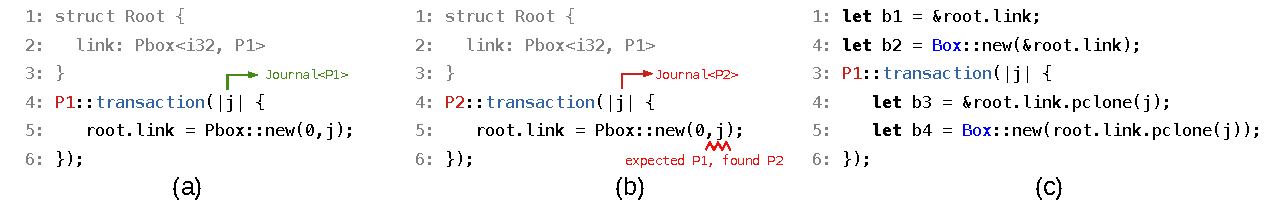
\includegraphics[width=7in]{Figures/links.pdf}
  \end{center}
  \caption{\label{fig:links} {\bf Different Links in \This{}.} (a) Legal assignment to an intra-pool pointer on line 5. (b) Illegal inter-pool pointer assignment; The \csym{Pbox} pointer at line 5 allocates memory from \csym{P2} and attempts to assign in to \csym{root.link} which is a \csym{P1} pointer. (c) A selection of Legal volatile to PM temporary pointers/borrows.}
\end{figure*}

\begin{figure}
  \begin{center}
  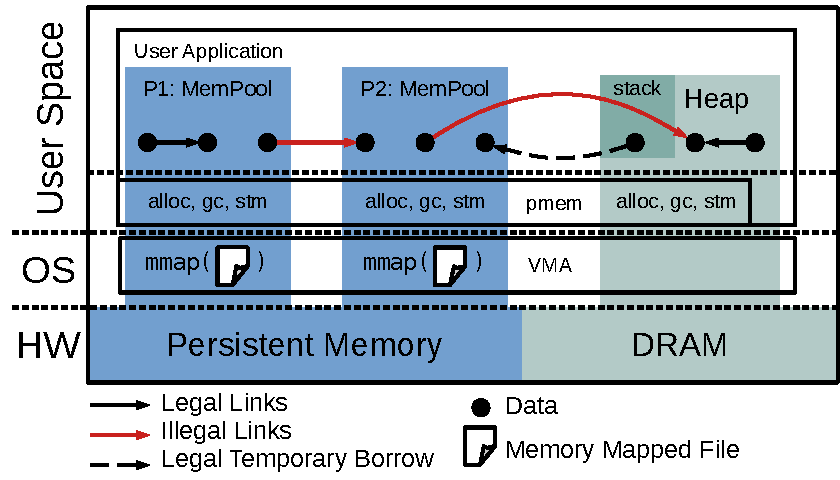
\includegraphics[width=3.2in]{Figures/stack.pdf}
  \end{center}
  \caption{\label{fig:stack} {\bf\this{}ic system stack.} Each \csym{MemPool} is associated with a memory mapped file. It provides memory management and logging interface. \csym{MemPool}s are isolated which means that inter-pool links are illegal. }
\end{figure}
}



% \refsec{sec:ptrs} describes how \This{} implements these constraints in detail. \steve{Do we have a `sec:ptrs' section?}

% \morteza{can we have inline code examples?  just a few lines.  It might be cleaner than using lstlisting.  Or we could have a single figure with (a), (b), (c), etc. for different short examples.}


%Allocation reversibility is required when we have a persistent memory and potentially system crashes to prevent persistent memory leakage. As explained in \refsec{sec:rust}, in Rust, variables drop their owned data when they go out of scope, and the memory occupied by objects is reclaimed when they are no longer in use. However, not only persistent objects may live longer than the program itself, but also they may remain in memory when the process unexpectedly is killed. Therefore, regular memory management mechanisms cannot handle persistent memory leaks.

%Reversible allocation ensures that the memory assigned to an object is not durable until it becomes reachable from the root object, and the transaction is committed. Otherwise, the allocation reverts on failure. The root object is the only persistent object that is accessible after re-opening the pool. \this{} makes sure that the allocation is reversible through a series of considerations. First, it takes a special kind of log for the allocation which indicates that `\textit{this allocation is not persistent}', before returning it. When a crash happens, it reverts the allocation using this log on recovery. Second, the allocator is not publicly visible to the user. Instead, \this{} provides persistent pointer wrappers that closely work with the allocator in background, and are available to the user. \refsec{sec:impl} discusses the details.
\lstDeleteShortInline^
